\section{Theoretical foundations}

This chapter is primarily based on the presentation by Sutton and Barto~\cite{Sutton2018}\footnote{All definitions and concepts not attributed to other sources are based on the exposition in Sutton and Barto (2018).}.

\subsection{\gls{RL} for Continuous Control}

\newacronym{MDP}{MDP}{Markov Decision Process}
\subsubsection{\gls{MDP}}

\begin{figure}[H] % Use figure* for full-width in twocolumn
    \centering
    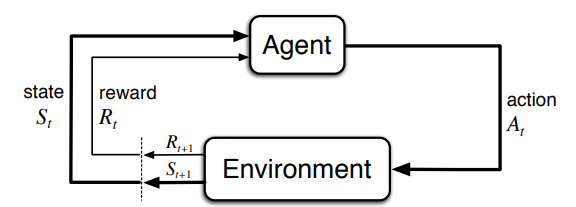
\includegraphics[width=0.45\textwidth]{MDP.png} % Passe den Dateinamen und Pfad an
    \caption{The agent environment interaction in a Markov decision process~\cite{Sutton2018}.}
    \label{fig:first} % For first figure
\end{figure}
\gls{RL} problems are typically formalized as \gls{MDP}s. An \gls{MDP} is defined by the tuple $(\mathcal{S}, \mathcal{A}, \mathcal{P}, \mathcal{R}, \gamma)$, where:

\begin{itemize}
    \item $\mathcal{S}$ is the state space,
    \item $\mathcal{A}$ is the action space,
    \item $\mathcal{P}$ is the transition probability distribution (or transition dynamics in the continuous case),
    \item $\mathcal{R}$ is the reward function,
    \item $\gamma \in [0,1]$ is the discount factor.
\end{itemize}

\noindent For continuous control problems, both $\mathcal{S}$ and $\mathcal{A}$ are continuous sets, typically represented as vectors of real values. Typically, the transition dynamics and reward functions are also continuous mappings. In continuous control, the transition dynamics are often described as a probability density over the next state.

\subsubsection{Agent, Environment, Reward and Policy}

Within this \gls{MDP}, \gls{RL} is considered in the context of an agent interacting with an environment over a sequence of time steps. This interaction can be formally described as shown in Figure~\ref{fig:first}:

\noindent At each time step~$t$:
\begin{itemize}
    \item The agent observes the current state $s_t \in \mathcal{S}$ of the environment,
    \item selects an action $a_t \in \mathcal{A}$ based on its policy,
    \item receives a reward $r_t \in \mathbb{R}$ from the environment, and
    \item transitions to a new state $s_{t+1}$.
\end{itemize}

\noindent The agent is the learning entity that aims to maximize the cumulative reward. It observes the environment through its state representation and acts according to its policy. Mathematically, the agent's objective is to maximize the expected return $G_t$, defined as the discounted sum of future rewards:

\begin{equation}
G_t = \sum_{k=0}^{\infty} \gamma^k r_{t+k+1}
\end{equation}

\noindent where $\gamma \in [0,1]$ is the discount factor, which determines the present value of future rewards.\\

\noindent The environment defines the dynamics of the system in which the agent operates. It determines how the state evolves and what reward is returned in response to the agent’s actions. Given a current state and an action taken by the agent, the environment produces the next state and the corresponding reward. This interaction captures the core feedback mechanism that enables learning in \gls{RL}.\\

\noindent The reward \( r_t \) is a scalar signal provided by the environment that indicates how good the agent’s action is in the current state. The reward function is formally defined as:

\begin{equation}
\mathcal{R}: \mathcal{S} \times \mathcal{A} \times \mathcal{S} \rightarrow \mathbb{R}
\end{equation}

\noindent where \( \mathcal{R}(s_t, a_t, s_{t+1}) \) represents the expected immediate reward when transitioning from state \( s_t \) to state \( s_{t+1} \) after taking action \( a_t \).\\

\noindent The policy \( \pi \) defines the agent’s strategy for selecting actions based on the current state. It guides the agent’s behavior by determining which action to take in each situation. In the case of a stochastic policy, \( \pi(a|s) \) represents the probability of taking action \( a \) given state \( s \). This allows the agent to explore different actions with varying likelihoods. For deterministic policies, the policy is a direct mapping from states to actions, written as:
\begin{equation} \pi(s) = a \end{equation}
Which means the agent always chooses the same action \( a \) in state \( s \).\\

\noindent The value function $V^\pi(s)$ represents the expected return when the agent starts in state $s$ and follows policy $\pi$:
\begin{equation} V^\pi(s) = \mathbb{E}_{\pi}\left[G_t \middle| S_t = s\right] \end{equation}
In continuous control problems the expectation is calculated over a continuous probability density of future states.\\

\noindent The action-value function $Q^\pi(s,a)$ represents the expected return when action $a$ is taken in state $s$ and policy $\pi$ is followed thereafter:
\begin{equation} Q^\pi(s,a) = \mathbb{E}_{\pi}\left[G_t \middle| S_t = s, A_t = a\right] \end{equation}
In continuous control problems, $a$ is a vector of continuous actions. The action-value function accounts for the probability density of transitions.\\

\noindent The optimal policy $\pi^*$ maximizes the expected return in every state:
\begin{equation} \pi^* = \arg\max_\pi V^\pi(s) \quad \forall s \in \mathcal{S} \end{equation}
For continuous control, the definition of the optimal policy remains the same, but policy $\pi^*$ provides a continuous action recommendation in each state.

\subsubsection{Differences Between Discrete and Continuous Action Spaces}

The fundamental difference between discrete and continuous action spaces lies in the number of possible actions available to the agent.

\noindent Discrete action spaces have a finite number of actions from which the agent can choose:
\begin{equation}
    \mathcal{A} = \{a_1, a_2, ..., a_n\}
\end{equation}
Examples are selecting one of four directions in a grid world or selecting a move in chess.\\
\noindent Continuous action spaces have actions from an uncountably infinite set, typically represented as real-valued vectors:
\begin{equation}
\mathcal{A} \subseteq \mathbb{R}^d
\end{equation}
where $d$ is the dimensionality of the action space. Examples are controlling joint torques in a robotic arm or adjusting steering and acceleration in a vehicle.\\

\noindent This results in several differences in algorithm design:

\begin{itemize}
    \item Exploration strategies:  Discrete spaces can use simple methods like  $\varepsilon$-greedy or softmax policies, while continuous spaces require adding noise to actions (\gls{DDPG} \cite{lillicrap2019continuouscontroldeepreinforcement}) or using stochastic policies that model probability distributions over actions (\gls{SAC} \cite{haarnoja2018softactorcriticoffpolicymaximum}, \gls{PPO} \cite{schulman2017proximalpolicyoptimizationalgorithms}).
    \item Action selection: Discrete actions use argmax operations over Q-values, where continuous actions involve sampling from stochastic policies or directly outputting values through specialized policy networks.
    \item Function approximation: Continuous action spaces need more advanced techniques to represent policies and value functions across infinite action domains \cite{fujimoto2018addressingfunctionapproximationerror}.
\end{itemize}

\subsubsection{Policy Gradient Methods}

Policy gradient methods are especially well-suited for continuous control problems because they optimize the policy parameters directly, without needing to discretize the action space. The main idea is to adjust the parameters $\theta$ of a parameterized policy $\pi_\theta$ in the direction of the expected return gradient\cite{wang2019neural}:

\begin{equation}
\nabla_\theta J(\pi_\theta) = \mathbb{E}_{\sigma_{\pi_\theta}} \left[ Q^{\pi_\theta}(s, a) \cdot \nabla_\theta \log \pi_\theta(a \mid s) \right]
\end{equation}

\noindent This is known as the policy gradient theorem, where $J(\theta)$ represents the expected return under the policy $\pi_\theta$:

\begin{equation}
J(\theta) = \mathbb{E}_{\pi_\theta} \left[G_0\right]
\end{equation}

\noindent For continuous action spaces, the policy $\pi_\theta(a|s)$ is often modeled as a Gaussian distribution:

\begin{equation}
\pi_\theta(a|s) = \mathcal{N}(\mu_\theta(s), \sigma_\theta(s))
\end{equation}

\noindent Here, $\mu_\theta(s)$ and $\sigma_\theta(s)$ are the mean and standard deviation of the action distribution.

%\noindent Actor-critic methods combine policy gradient techniques with value function approximation. In this setup, an actor network learns the policy, while a critic network estimates the action values or advantages.

\subsection{Function Approximation in \gls{RL}}

In continuous control tasks, both the state and action spaces are continuous, making it impractical to represent value functions or policies using tabular methods. The function approximation, particularly with neural networks, has become the standard approach to manage the complexity and dimensionality in these problems~\cite{gottwald2018neuralvalue}.

\subsubsection{Neural Networks as Function Approximators}

Neural networks serve as universal function approximators, capable of modeling complex relationships between continuous states and actions. In continuous control settings, they are typically utilized in two primary roles:
\begin{itemize}
    \item Value function approximation: Neural networks estimate state value functions $V(s)$ or action value functions $Q(s, a)$, mapping continuous inputs to scalar outputs~\cite{gottwald2018neuralvalue}.
    \item Policy approximation: Networks directly parameterize policies, which can be:
    \begin{itemize}
        \item \textit{Deterministic:} Outputting specific continuous actions.
        \item \textit{Stochastic:} Outputting parameters of probability distributions over actions~\cite{gottwald2018neuralvalue}.
    \end{itemize}
\end{itemize}

\noindent The flexibility of neural networks allows them to capture non-linear dependencies, which makes them well suited for continuous control problems such as those found in robotics~\cite{gottwald2018neuralvalue}.

\subsubsection{Challenges in Representing Continuous Policies}

Representing policies in continuous action spaces introduces several unique challenges.
\begin{itemize}
    \item Output representation:  Neural networks must produce outputs within feasible ranges for each action dimension, enforced using bounded activation functions (e.g. \texttt{ tanh}) or by post-processing outputs~\cite{wang2018explorationexploitation}.
    \item Exploration-exploitation tradeoff: Exploration in continuous spaces relies on adding Gaussian noise to deterministic policies or sampling from learned stochastic policies~\cite{wang2018explorationexploitation}.
    \item Training stability: Minor parameter changes can lead to large behavioral differences, requiring techniques such as gradient clipping, target networks, and conservative policy updates to stabilize learning~\cite{shen2024ddpgtd3walker2d}.
\end{itemize}

\subsubsection{Actor-Critic Architecture Overview}

The actor-critic architecture is fundamental in modern continuous control algorithms. It comprises two interacting neural networks:

\begin{figure}[H] % Use figure* for full-width in twocolumn
    \centering
    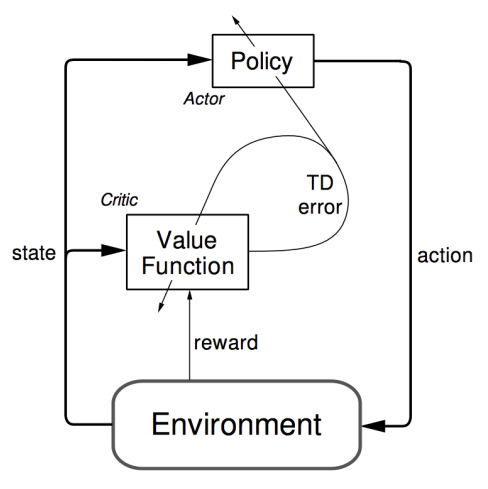
\includegraphics[width=0.45\textwidth]{actorcritic.png} % Passe den Dateinamen und Pfad an
    \caption{Scheme of information flows in actor-critic agent \cite{Sutton2018}.}
    \label{fig:mdp}
\end{figure}

\begin{itemize}
    \item Actor network: Represents the policy $\pi(a|s)$, mapping states to actions. For continuous actions, the actor typically outputs either: \begin{itemize}
        \item Mean and standard deviation for a Gaussian policy, or
        \item Direct deterministic action values.
    \end{itemize}
    \item Critic network: Estimates value functions, providing a learning signal to guide actor updates.
    %such as $Q(s, a)$ or the advantage function $A(s, a)$
\end{itemize}

\noindent This dual network system improves training stability compared to pure policy gradient methods. The critic reduces the variance of the gradient, while the actor allows efficient optimization of continuous actions~\cite{Sutton2018}. The actor-critic framework forms the basis for many state-of-the-art algorithms in continuous control, including \gls{DDPG}, \gls{PPO}, and \gls{SAC}, which we will examine in detail in the following section.
